\documentclass[10pt,letterpaper]{article}
\usepackage[lmargin=2.2in,rmargin=0.7in,tmargin=1.0in,bmargin=1.0in]{geometry}
\usepackage{notes}
\begin{document}


\begin{center}
\Large\textbf{2.3 - Characteristic Equation: Repeated Roots}\\
\normalsize (Section 2.2.2)
\end{center}

%-------------------------------------------------------------
\section{The Issue with Repeated Roots}
Let's first go over what the issue is with repeated roots.

\subsection{Characteristic Equation Method}
Here are the steps to solve the second order IVP
\[
\begin{dcases}
ax''+bx'+cx=0,\\
x(0)=x_0,\\
x'(0)=v_0.
\end{dcases}
\]

\begin{enumerate}
    \item First write the characteristic equation
\[
a\lambda^2+b\lambda+c=0.
\]
    \item Solve for the eigenvalues $\lambda_1$ and $\lambda_2$.
    \item Write the general solution as the linear combination
    \[
    x(t)=C_1e^{\lambda_1t}+C_2e^{\lambda_2t}.
    \]
    \item Use the initial conditions to solve for $C_1$ and $C_2$.\\
\end{enumerate}
\textbf{Warning}: these steps only apply when the two eigenvalue $\lambda_1$ and $\lambda_2$ are real and distinct.

% -----------

\subsection{Wrong Attempt}
Consider the problem 
\[
\begin{dcases}
x''-4x'+4x=0, \\
x(0) = 1,\\
x'(0)=0.
\end{dcases}
\]
The characteristic equation can be factored cleanly, giving us two eigenvalues $\lambda_1=\lambda_2=2$. 
\[
\lambda^2-4\lambda+4=0
\quad\Rightarrow\quad
(\lambda-2)(\lambda-2)=0.
\]
If we naively follow the steps, our general solution is
\[
x(t)=C_1e^{2t}+C_2e^{2t}.
\]
The condition $x(0)=1$ says $C_1+C_2=1$. The condition $x'(0)=0$ says $2C_1+2C_2=0$. However, this linear system 
$$
\begin{dcases}
    C_1+C_2=1\\
    2C_1+2C_2=0 
\end{dcases}
$$
has \textit{no solutions}; it's inconsistent. But the existence and uniqueness theorem tells us that this IVP must have a solution. We made a grave mistake somewhere in this calculation.

% ------------

\subsection{What Went Wrong?}

Recall that the combination 
\[
x(t)=C_1x_1(t)+C_2x_2(t)
\]
is only a general solution if the two functions $x_1$ and $x_2$ are \textit{independent}. In the previous example, we only had one eigenvalue $\lambda=2$ and one solution
\[
x_1(t)=e^{2t}.
\]
The mistake was that our second solution was the same as our first $x_2=x_1$.
In fact, because $C_1$ and $C_2$ are both arbitrary, they just combine as one:
\[
C_1e^{2t}+C_2e^{2t}
=(C_1+C_2)e^{2t}
=\widetilde{C}e^{2t}.
\]
Adding a second dependent solution adds no contribution to the solution. When you have repeated eigenvalues, you must find a second independent solution.

%%%%%%%%%%%%%%%%%%%%%%%%%%%%%%%%%%%%%%%%%%%%%%%%%%%%%%%%%%%%%%%%%%%%%%%%

\section{The Proper Method}
Now we will explain how to properly solve the DE in the case of repeated eigenvalues.

\subsection{General Solution}
Suppose the characteristic equation has a repeated real root $\lambda$.
Then one solution is
\[
x_1(t)=e^{\lambda t}.
\]
To obtain a second independent solution $x_2$, we multiply the solution $x_1$ by $t$:
\[
x_2(t)=t\,x_1(t)=te^{\lambda t}.
\]
Thus, the general solution is the combination of $x_1$ and $x_2$
\[
x(t)=C_1e^{\lambda t}+C_2te^{\lambda t}.
\]
This is a rather non-intuitive result. The next section shows the proof of why this works. You will not be tested on the proof.

%--------------------------------------------
\subsection{Proof (Optional Reading)}
We already know the solution $e^{\lambda t}$. To find another,
try $x(t)=v(t)e^{\lambda t}$. Differentiating gives
\begin{align*}
x'  &= (v'+\lambda v)e^{\lambda t},\\
x'' &= (v''+2\lambda v'+\lambda^2v)e^{\lambda t}.
\end{align*}
Substitute into $ax''+bx'+cx=0$ and divide by $e^{\lambda t}$:
\[
av''+(2a\lambda+b)v'+(a\lambda^2+b\lambda+c)v=0.
\]
Since $\lambda$ is a repeated root,
\[
a\lambda^2+b\lambda+c=0,
\qquad
\lambda=-\frac{b}{2a}
\quad\Rightarrow\quad
2a\lambda+b=0.
\]
Thus, the equation reduces to
\[
av''=0
\quad\Rightarrow\quad
v''=0
\quad\Rightarrow\quad
v(t)=A+Bt.
\]
Therefore,
\[
x(t)=(A+Bt)e^{\lambda t}
=Ae^{\lambda t}+Bte^{\lambda t}.
\]
The factor of $t$ appears naturally when we integrate $v''=0$ twice. Now we can return to the previous IVP and solve it correctly.

%-------------------------------------------------------------
\begin{example}[1]{
Find the solution to
\[
\begin{dcases}
x''-4x'+4x=0, \\
x(0) = 1,\\
x'(0)=0.
\end{dcases}
\]
}
Since the eigenvalue is a repeated root $\lambda=2$, we write the general solution as  
\[
x(t)=C_1 e^{2t}+C_2 \,t\,e^{2 t}.
\]
The condition $x(0)=1$ gives
\[
C_1=1.
\]
Therefore,
\[
x(t)=e^{2t}+C_2te^{2t}.
\]
The derivative is
$$
x'(t) = (e^{2t}+C_2 \,t\,e^{2 t})' = 2e^{2t}+C_2(e^{2t}+2te^{2t}).
$$
Therefore, the condition $x'(0)=0$ yields 
$$
x'(0)=2+C_2(1+0) = 0 \implies C_2 = -2.
$$
Therefore the solution is 
$$
\boxed{
x(t) = e^{2t} - 2te^{2t}.
}
$$
This is the unique solution that exists for all $t\in \mathbb{R}$ as guaranteed by our well-posedness theorem.
\end{example}

%%%%%%%%%%%%%%%%%%%%%%%%%%%%%%%%%%%%%%%

\section{Sketching the Solution}
Our goal is to learn how to sketch the repeated-root solution by hand.

% ----------

\subsection{Sketching Strategy}

Repeated-root solutions have the form
\[
x(t)=(C_1+C_2t)e^{\lambda t},
\]
which is ``linear times exponential.'' As in the previous lecture,
we use the initial conditions and end behavior to guide our sketch:
\begin{enumerate}
    \item Plot the initial point $(0,x_0)$ and indicate
    the initial slope $x'(0)=v_0$.
    \item Find the zero by solving $C_1+C_2t=0$, if it exists.
    \item Determine the behavior as $t\to\infty$ and $t\to-\infty$.
    \item Connect these features using the shape of
    a linear function times an exponential.
\end{enumerate}
To understand this shape, let's first look at a simple example.

% ----------

\subsection{General Shape}

Consider the function
\[
x(t)=te^{-t}.
\]
This function is the product of a linear function $t$ and an exponential
$e^{-t}$. As $t$ increases, the linear factor grows while the
exponential factor decays. 
Therefore, direct substitution into the product gives the indeterminate
form
\[
\lim_{t\to\infty} te^{-t} =\infty\cdot0.
\]
You may use L'Hopital's rule to verify that
\[
te^{-t}\to0
\qquad\text{as }t\to\infty.
\]
Towards the other end, we have
\[
te^{-t}\to-\infty
\qquad\text{as }t\to-\infty.
\]
The resulting graph has a characteristic ``bump-and-decay'' shape.
This is a useful prototype for understanding repeated-root solutions.
\begin{figure}[H]
    \centering
    \begin{tikzpicture}[scale=0.9]
    % axes
    \draw[->,thick] (-1,0) -- (5,0) node[right] {$t$};
    \draw[->,thick] (0,-2) -- (0,2) node[above] {$x$};
    \draw[thick,domain=-0.4:5,samples=200]
    plot (\x,{3*\x*exp(-1.2*\x)});
\end{tikzpicture}\caption{ Sketch of $x(t)=t\,e^{-t}$. }
\end{figure}


\begin{example}[2]{
Sketch the function
\[
x(t)=e^{2t}-2te^{2t},
\]
which satisfies the initial conditions
$x(0)=1$ and $x'(0)=0$.
}
One of the intercepts is given $(0,1)$. To find the other intercept, factor out $e^{2t}$ and find the root of the linear factor:
\begin{align*}
x(t)&=    e^{2t} - 2te^{2t}\\
&=e^{2t}(1-2t) \equiv0\\
&\implies (1-2t)=0\\
&\implies t=1/2
\end{align*}
Begin by plotting the two points $(0,1)$ and $(0.5,0)$. Since $x'(0)=0$, indicate a horizontal tangent at the point $(0,1).$ Next, calculate the limits:
$$
 \lim_{t\rightarrow \infty} x(t) =  \lim_{t\rightarrow \infty} e^{2t}(1-2t) = -\infty,
$$
$$
 \lim_{t\rightarrow -\infty} x(t) =\lim_{t\rightarrow -\infty} e^{2t}(1-2t) = 0.
$$
Lastly, put all the information together. Draw a bump that peaks at $(0,1)$ which decays as we move left. To the right, it passes through $(0.5,0)$ and sinks to $-\infty$.
\begin{figure}[H]
    \centering
    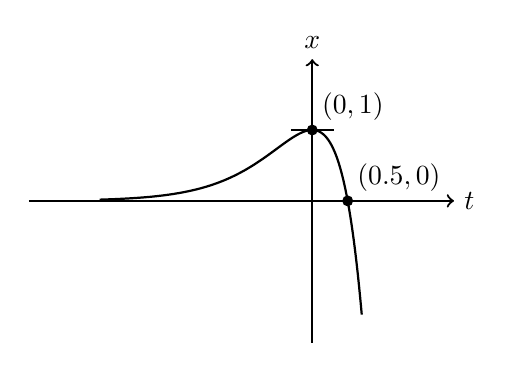
\begin{tikzpicture}[scale=0.9]
    % axes
    \draw[->,thick] (-4,0) -- (2,0) node[right] {$t$};
    \draw[->,thick] (0,-2) -- (0,2) node[above] {$x$};

    \draw[thick,domain=-3:0.7,samples=200]
    plot (\x,{(-2*\x+1)*exp(2*\x)});

    \fill (0,1) circle (2.2pt);
    \fill (0.5,0) circle (2.2pt);
    \node[above right] at (0,1) {$(0,1)$};
    \node[above right] at (0.5,0) {$(0.5,0)$};

    \draw[thick] (-0.3,1) -- (0.3,1);
\end{tikzpicture}\caption{ Sketch of $x(t)=(-2t+1)\,e^{2t}$}
    \label{fig:placeholder}
\end{figure}
\end{example}


% --------------------------------------------------
\section{From Solution to IVP}

So far, we have started with an IVP and found its solution. Can we go
in reverse? If we are given a repeated-root solution, can we construct
an IVP that produces it?

Yes. In fact, this is how I sometimes construct exam
problems with nice, clean solutions. This is mostly a fun exercise, but it is on your homework, so let's see how it works.

\subsection{General Steps}

Suppose we are given a repeated-root solution
\[
x(t)=(C_1+C_2t)e^{r t}.
\]
We can recover an IVP using the following steps:
\begin{enumerate}
    \item Write the characteristic equation in factored form:
    \[
    (\lambda-r)^2=0.
    \]

    \item Expand:
    \[
    \lambda^2-2r\lambda+r^2=0.
    \]

    \item Convert the characteristic equation into a differential equation:
    \[
    x''-2rx'+r^2x=0.
    \]

    \item Find the initial position by evaluating $x(0)$.

    \item Find the initial velocity by evaluating $x'(0)$.
\end{enumerate}

\begin{example}[3]
{
Find an IVP whose solution is given by $$x(t)=2e^{4t}-te^{4t}.$$
}
The characteristic equation is 
\begin{align*}
    0 &= (\lambda-4)^2\\
    0 &= \lambda^2 -8\lambda + 16
\end{align*}
so the coefficients are $a=1$, $b=-8$, and $c=16$. One possible differential equation is
$$
x'' -8x' +16x=0.
$$
Plugging in $t=0$ gives 
$$
x(0) = 2e^{0}-(0)e^{0}=2
$$
which must be the value of $x_0$. Taking the derivative gives us 
$$
x'(t) = 8e^{4t} -(e^{4t}+4te^{4t}).
$$
Plugging in $t=0$ into the derivative gives 
$$
x'(0) = 8e^{0} -(e^{0}+4(0)e^{0}) = 8-1=7
$$
which must be the value of the initial derivative. One IVP would be  
$$
\boxed{
\begin{dcases}
x''-8x'+ 16x=0, \\
x(0) = 2,\\
x'(0)=7
\end{dcases}.
}
$$
\end{example}

%%%%%%%%%%%%%%%%%%%%%%%%%%%%%%%%%%%%%%%%%%%%%%%%%%%%%%%%
\section{Complex Numbers}
Since we have time to spare, we can begin discussing the third case: complex eigenvalues.

\subsection{Non-real Roots}

Consider the DE
\[
x''-2x'+5x=0.
\]
The characteristic equation is
\[
\lambda^2-2\lambda+5=0.
\]
We can solve it using the quadratic formula, but we encounter a complication
\[
\lambda
=\frac{-b\pm\sqrt{b^2-4ac}}{2a}
=\frac{2\pm\sqrt{4-20}}{2}
=1\pm\frac{1}{2}\sqrt{-16}.
\]
The issue is that $\sqrt{-16}$ is not a real number. More precisely,
\[
\text{there is no $x\in\mathbb{R}$ such that }x^2=-16.
\]
The roots do exist, just not in $\mathbb{R}$. We need to introduce a broader class of numbers that allows us to solve equations such as $x^2+16=0$.

% ------ 

\subsection{Imaginary Unit}

We define the \textbf{imaginary unit} $i$ to be
\[
i=\sqrt{-1}.
\]
The imaginary unit is not a real number, so $i\notin\mathbb{R}$.
It belongs to a larger number system called the \textbf{complex numbers},
denoted by $\mathbb{C}$. This new number satisfies
\[
i^2=-1.
\]
We can perform ordinary algebra with $i$. For example,
\[
i+2i=3i,
\qquad
(2i)(3i)=6i^2=-6.
\]
More importantly, $i$ allows us to write square roots of negative
numbers. For example,
\[
\sqrt{-16}=\sqrt{(-1)(16)}=4i.
\]
For our purposes, this is really all we need to know about $i$.
Now we can return to our differential equation.


\begin{example}[4]
{
Find the \textit{complex} eigenvalues for
\[
x''-2x'+5x=0.
\]
}
From the previous subsection, the characteristic equation gives
\[
\lambda
=1\pm\frac{1}{2}\sqrt{-16}.
\]
Using the imaginary unit,
\[
\sqrt{-16}=4i,
\]
so
\[
\lambda
=1\pm\frac{1}{2}(4i)
=1\pm2i.
\]
Therefore, the two complex eigenvalues are
\[
\boxed{\lambda_1=1+2i,
\qquad
\lambda_2=1-2i.}
\]

\end{example}

% --------- 

\subsection{Standard Form}

Any complex number $z\in\mathbb{C}$ can be written in the form
\[
z=a+ib,
\]
where $a,b\in\mathbb{R}$. This is called the \textbf{standard form}
of a complex number. The term $a$ is called the \textbf{real part}, while $b$ is called the
\textbf{imaginary part}. For example,
\[
z=3+2i
\]
has real part $3$ and imaginary part $2$. Sometimes, it is not so obvious what the real and imaginary parts are. Some algebraic manipulation may be required. Consider the number $z=5i+2/i$. To see what the real and imaginary parts are, multiply the 2nd term by $i/i$:
\begin{align*}
    z &= 5i+\frac{2}{i}\frac{i}{i}\\
     &= 5i+\frac{2i}{i^2}\\
     &= 5i-2i\\
     &= 3i
\end{align*}
For this complex number, the real part is $0$ and the imaginary part is $3$. 
    
% ----- 

\subsection{Euler's Formula}
Complex numbers can appear in the exponential function. In this case, writing the number in standard form requires the help of a theorem.

\begin{theorem}
If $i=\sqrt{-1}$ then for any $t\in\mathbb{R}$,
\[
e^{it}=\cos t+i\sin t.
\]
\end{theorem}

This equation is called \textbf{Euler's formula}. Here is a simple use of the formula:
\[
e^{i\pi/2}
=
\cos\frac{\pi}{2}
+i\sin\frac{\pi}{2}
=i.
\]
The main use of Euler's formula for us is to write complex exponential functions in standard form so that we can identify their real and imaginary parts.


\begin{example}[6]{
Write the number
$$
z = e^{6+3i}
$$
in the standard form $z=a+ib$.
}
Rewrite the exponential as a product and apply Euler's formula
\begin{align*}
z &= e^{6+3i}\\
 &= e^6e^{3i}\\
 &= e^6(\cos(3)+i\sin(3))\\
 &= e^6\cos(3)+ie^6\sin(3)
\end{align*}
The standard form is 
$$
    \boxed{z=e^6\cos(3)+ie^6\sin(3).}
$$
Thus, the real part is $e^6\cos(3)$ and the imaginary part is $e^6\sin(3).$
\end{example}

\subsection{Odd and Even Functions}
What would the number
$$
    z = e^{6-3i}
$$
look like when it is written in standard form? Using Euler's formula, we get 
\begin{align*}
z &= e^{6-3i}\\
 &= e^6e^{-3i}\\
 &= e^6\cos(-3)+ie^6\sin(-3)
\end{align*}
We can clean this up a bit. Recall that $\cos(x)$ is an even function, i.e. 
$$
    \cos(-x) =\cos(x)
$$
and that $\sin(x)$ is an odd function, i.e. 
$$
    \sin(-x) = -\sin(x).
$$
Therefore 
$$
z = e^{6-3i} = e^6\cos(3)-ie^6\sin(3)
$$
\subsection{Next Lecture}
In Example 4, we found that
\[
x''-2x'+5x=0
\]
has eigenvalues $\lambda=1\pm2i$. As before, the eigenvalue
$\lambda=1+2i$ gives an exponential solution
\[
x_1(t)=e^{(1+2i)t}.
\]
However, this solution is complex-valued, while we want real
solutions. Next lecture, we will use Euler's formula to obtain
the real general solution.

\end{document}
